% Conditional Strategies II -- timing expected returns: the dividend yield for the market, the value spread for factors,
% why in-sample evidence misleads, and 24 factor signals.
% Figures and every number quoted here come from conditional_strategies_figures.py, except appendix A3 (the value spread at
% today's prices), which comes from the check at the end of chapters/Finance/build_value_spread_data.py
% Companion notebook: chapters/Finance/L15_ConditionalStrategiesII_AI.ipynb (exercises 1-5 in class, the challenge is homework)
% Structure: content first, then one slide per notebook exercise, then takeaways.
% The challenge answer (the out-of-sample R2 for D/P with forecasts from 1980) must not appear here: this PDF is public.
\documentclass[aspectratio=169,10pt]{beamer}
\usetheme{default}
\usecolortheme{default}

\usepackage{graphicx}
\usepackage{adjustbox}
\usepackage{amsmath}
\usepackage{amssymb}
\usepackage{booktabs}
\usepackage{array}
\usepackage{tikz}
\usetikzlibrary{arrows.meta,positioning,calc,decorations.pathreplacing}
\usepackage{appendixnumberbeamer}  % Exclude appendix from slide count

\setbeamertemplate{navigation symbols}{}
\setbeamertemplate{items}[circle]

% Footline: Author, Event (Year) on left; page/total on right
\setbeamertemplate{footline}{
  \hbox{%
    \begin{beamercolorbox}[wd=.5\paperwidth,ht=2.5ex,dp=1ex,left]{author in head/foot}%
      \hspace*{2ex}\insertshortauthor, \insertshortinstitute\ (\insertdate)
    \end{beamercolorbox}%
    \begin{beamercolorbox}[wd=.5\paperwidth,ht=2.5ex,dp=1ex,right]{date in head/foot}%
      \insertframenumber/\inserttotalframenumber\hspace*{2ex}
    \end{beamercolorbox}%
  }
}

% Highlight boxes
\setbeamercolor{box1}{bg=red!12,fg=black}

% A poll option: {colour}{letter and choice}
\newcommand{\pollbox}[2]{\tikz\node[draw=#1!65!black, fill=#1!10, rounded corners=4pt, minimum width=3.7cm,
                                   minimum height=1.0cm, align=center, font=\normalsize]{#2};}
\newcolumntype{P}[1]{>{\raggedright\arraybackslash}p{#1}}

\title{Conditional Strategies II}
\subtitle{Timing expected returns}
\author[A. Moreira]{Alan Moreira}
\institute[Data-Driven Investing]{NYU Stern --- Data-Driven Investing}
\date{Fall 2026}

\begin{document}

\begin{frame}
\titlepage
\end{frame}

%================================================================== INTRODUCTION
\begin{frame}{Value is cheap. The market is not.}
\vskip 6pt
\begin{itemize}
\item June 2026: value stocks' book-to-market was \textcolor{red}{9.5} times growth stocks'. Usually it is 5. The last time the gap was this wide: 1943.
\vskip 8pt
\item The market: dividends were 1.6\% of its price at the end of 2024, lower than in 93\% of months since 1926
\vskip 8pt
\item If a low price means a high future return, you would hold more value and less of the market. Should you?
\vskip 8pt
\item Today: do prices forecast returns, for the market and for factors, and how to check before you bet
\end{itemize}
\vskip 14pt
\begin{beamercolorbox}[rounded=true,sep=7pt,center]{box1}
Last class you forecast risk. Today you forecast the return itself: the hard part.
\end{beamercolorbox}
\end{frame}

\begin{frame}{Last class we timed $\sigma$. Today, $\mu$.}
\[ x_{t} \;=\; \frac{1}{\gamma}\,\frac{\mu_{t}}{\sigma_{t}^{2}} \]
\vskip 4pt
\begin{itemize}
\item Volatility forecast itself: last month explained half of this month
\vskip 8pt
\item Expected returns are the hard half. A mean needs decades to learn (\emph{Backtesting}), and the optimizer magnifies its errors (\emph{Capital Allocation III})
\vskip 8pt
\item The natural candidates: prices against fundamentals. For the market, its dividends. For a factor, the book values of what it buys and what it sells.
\end{itemize}
\vskip 14pt
\begin{beamercolorbox}[rounded=true,sep=7pt,center]{box1}
Is there a signal that tells you when an asset will pay more?
\end{beamercolorbox}
\end{frame}

%================================================================== THE MARKET: D/P
\begin{frame}{The classic signal: prices against dividends}
\begin{columns}[c]
\begin{column}{0.60\textwidth}
\adjustbox{max width=\textwidth, max height=0.70\textheight}{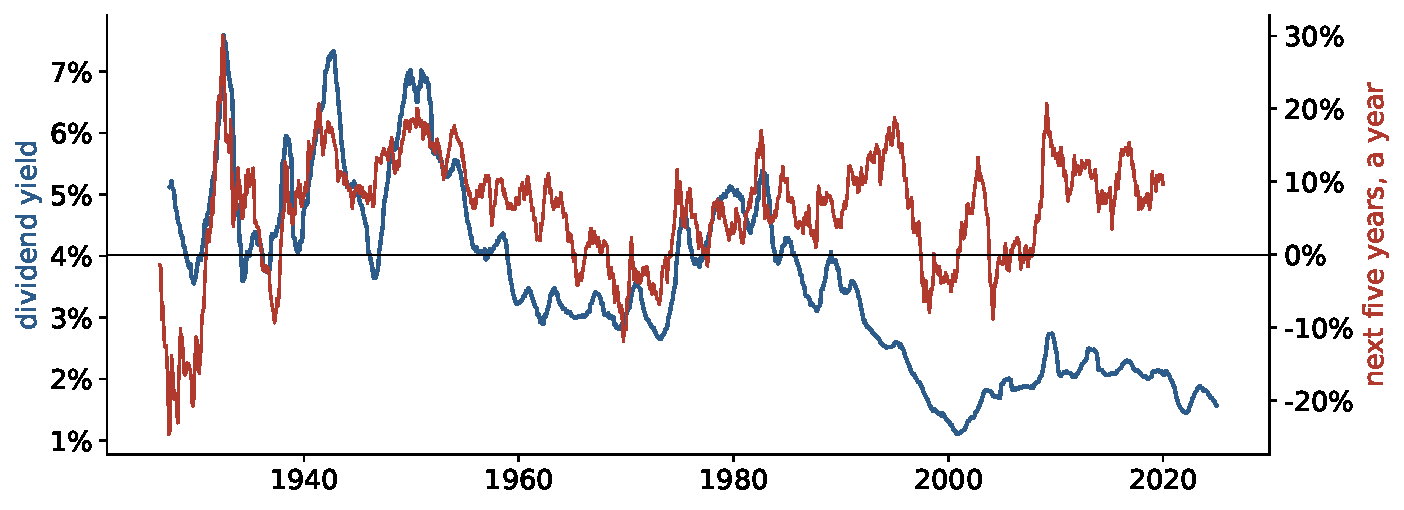
\includegraphics{figures/cs_dp.pdf}}
\end{column}
\begin{column}{0.38\textwidth}
From the Gordon model, $P = D/(r-g)$:
\[ \frac{D}{P} \;=\; r - g \]
\begin{itemize}
\item Low prices against dividends mean high future returns, or low future growth
\vskip 6pt
\item Correlation with the next five years' return: \textcolor{red}{0.35}
\vskip 6pt
\item Shiller's Nobel was for this pattern
\end{itemize}
\end{column}
\end{columns}
\end{frame}

\begin{frame}[label=reg]{The regression, at three horizons}
\[ r_{t \to t+h} \;=\; a \;+\; b\cdot \frac{D}{P}\Big|_{t} \;+\; u_{t+h} \]
{\small $r_{t\to t+h}$: the market's return over the next $h$ months, a year, over T-bills. D/P: last 12 months of dividends over today's price.}
\vskip 6pt
\begin{center}
\renewcommand{\arraystretch}{1.3}
\begin{tabular}{lccc}
\toprule
1927--2024 & next month & next year & next five years \\
\midrule
$b$ & 2.3 & 2.4 & 1.8 \\
$t$, as usually computed & 1.8 & 6.2 & \textcolor{red}{12.3} \\
$R^{2}$ & 0.3\% & 3.2\% & \textcolor{red}{12.1\%} \\
\bottomrule
\end{tabular}
\end{center}
\vskip 8pt
\begin{itemize}
\item The longer the horizon, the better it looks. A 12\% $R^{2}$ for stock returns would be remarkable.
\vskip 4pt
\item So remarkable that you should ask what is wrong
\end{itemize}
\end{frame}

\begin{frame}{Overlap fakes significance}
\vskip 4pt
\begin{center}
\renewcommand{\arraystretch}{1.3}
\begin{tabular}{lccc}
\toprule
 & next month & next year & next five years \\
\midrule
observations & 1,170 & 1,159 & 1,111 \\
of which do not overlap & 1,170 & 96 & \textcolor{red}{18} \\
\midrule
$t$, as usually computed & 1.8 & 6.2 & 12.3 \\
$t$, allowing for overlap (HAC) & 1.3 & 2.2 & \textcolor{red}{2.8} \\
\bottomrule
\end{tabular}
\end{center}
\vskip 8pt
\begin{itemize}
\item Two five-year returns a month apart share 59 of their 60 months. They are almost the same observation.
\vskip 4pt
\item Using only five-year periods that do not overlap: 19 observations, $t = 1.5$
\end{itemize}
\vskip 8pt
\begin{beamercolorbox}[rounded=true,sep=7pt,center]{box1}
A century of data is about 20 independent five-year returns
\end{beamercolorbox}
\vskip 2pt
\hfill \hyperlink{appendix_hac}{\beamerbutton{HAC, in a picture}}
\end{frame}

\begin{frame}{Poll}
\vskip 14pt
\begin{center}
{\large D/P explains 0.3\% of next month's return.\\[4pt] Suppose that is real, and you trade on it.}
\vskip 18pt
How much better is your Sharpe ratio than 0.40?
\vskip 18pt
\pollbox{gray}{\textbf{A}\ \ no better} \hfill
\pollbox{red}{\textbf{B}\ \ about 0.44} \hfill
\pollbox{blue}{\textbf{C}\ \ about 0.80}
\end{center}
\end{frame}

\begin{frame}[label=ct]{A small $R^{2}$ can be worth a lot}
Campbell and Thompson (2008): if the signal is real, with monthly $R^{2}$,
\[ SR^{2}_{\text{timed}} \;\approx\; \frac{SR^{2} + R^{2}}{1 - R^{2}} \qquad \text{(monthly units)} \]
\vskip 2pt
\begin{center}
\renewcommand{\arraystretch}{1.25}
\begin{tabular}{lccc}
\toprule
monthly $R^{2}$ & 0.3\% & 1\% & 2\% \\
\midrule
Sharpe ratio a year, from 0.40 & \textcolor{red}{0.44} & 0.53 & 0.64 \\
\bottomrule
\end{tabular}
\end{center}
\vskip 8pt
\begin{itemize}
\item The poll's answer is B. A monthly $R^{2}$ of 1\% is worth a third more Sharpe ratio.
\vskip 4pt
\item So small $R^{2}$s are not the problem. Whether they are real is.
\end{itemize}
\hfill \hyperlink{appendix_ct}{\beamerbutton{Where it comes from}}
\end{frame}

\begin{frame}[label=compare]{What is the right comparison?}
To see if it is real, trade the forecast. Each month from 1950, fit on the past only, then hold
\[ x_{t} \;=\; \frac{1}{\gamma}\,\frac{\text{forecast}_{t}}{\sigma^{2}} \quad \text{of the market, and the rest in T-bills} \]
{\small $\gamma = 3$. $\sigma^{2}$: the market's variance before 1950, held fixed.}
\vskip 8pt
Timing has to beat \emph{not timing}: a constant position in the market. How large?
\vskip 4pt
\begin{itemize}
\item \textbf{The same average position}, $\bar{x}$. The same money in the market on average: timing wins only if it held more before the good months.
\vskip 6pt
\item \textbf{The same beta}, $\beta$. The same exposure to the market's moves. It differs from $\bar{x}$ if the position is larger in volatile months.
\end{itemize}
\vskip 8pt
\begin{beamercolorbox}[rounded=true,sep=7pt,center]{box1}
In the end it is the alpha question again: does timing have alpha against buy and hold? \\[3pt]
$r^{\text{timing}}_{t} \;=\; \alpha + \beta\, r_{t} + \varepsilon_{t}$
\end{beamercolorbox}
\end{frame}

\begin{frame}{Out of sample, the edge is one episode}
\begin{center}
\adjustbox{max width=\textwidth, max height=0.50\textheight}{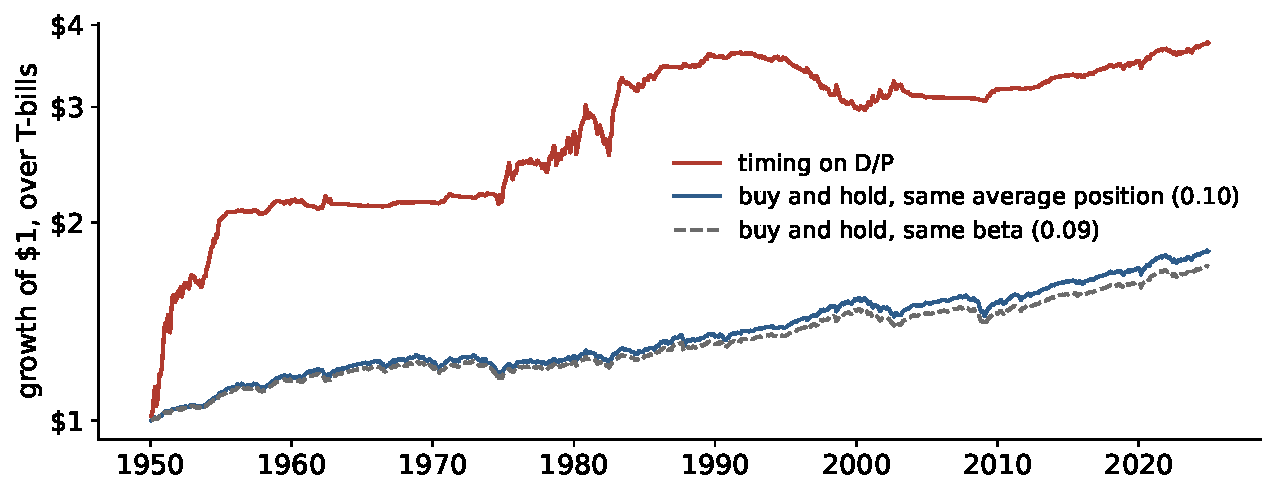
\includegraphics{figures/cs_timing.pdf}}
\end{center}
\begin{itemize}
\item Alpha against the market: \textcolor{red}{1.1\% a year, $t = 2.6$}. The two buy-and-holds nearly coincide.
\vskip 4pt
\item But \textcolor{red}{78\%} of that gap was earned by 1955: a position of 0.63 on average, while the market made 19\% a year. From 1956: alpha 0.5\% a year, $t = 1.3$
\vskip 4pt
\item And as a forecast, D/P loses to the historical average. Out-of-sample $R^{2}$: $-0.5\%$. 1950--1979: $+1.6\%$. 1980--1999: $-3.3\%$. 2000--2024: $-0.2\%$
\end{itemize}
\end{frame}

\begin{frame}{Trading it: great until 1990, then not}
\vskip 4pt
\begin{center}
\renewcommand{\arraystretch}{1.35}
\begin{tabular}{lcc}
\toprule
out of sample, Sharpe ratio & timing on D/P & buy and hold \\
\midrule
1950--1979 & \textcolor{red}{0.70} & 0.53 \\
1980--1999 & \textcolor{red}{0.13} & 0.63 \\
2000--2024 & 0.53 & 0.43 \\
\midrule
1950--2024 & 0.46 & 0.52 \\
\bottomrule
\end{tabular}
\end{center}
\vskip 10pt
\begin{itemize}
\item The weight is the forecast over $\gamma\sigma^{2}$. It was short the market in 36\% of months.
\vskip 6pt
\item D/P fell from about 4\% in the 1980s to about 1\% by 2000, and the regression read every year of it as \emph{sell}
\vskip 6pt
\item Through one of the best two decades for stocks in the sample
\end{itemize}
\end{frame}

\begin{frame}{What broke}
\vskip 8pt
\begin{itemize}
\item \textbf{Firms pay out differently.} Since the 1980s, buybacks have replaced dividends. The same payout now shows up as a lower D/P.
\vskip 10pt
\item \textbf{The premium may have fallen.} If investors now accept less, D/P settles at a lower level, and a regression fit on the past reads it as a permanent signal to sell.
\vskip 10pt
\item \textbf{Either way, the signal's average moved.} A forecasting regression assumes it does not.
\end{itemize}
\vskip 14pt
\begin{beamercolorbox}[rounded=true,sep=7pt,center]{box1}
The relationship was never estimated precisely enough to survive a change in its average
\end{beamercolorbox}
\end{frame}

\begin{frame}{D/P is one candidate among many}
\begin{center}
\footnotesize
\renewcommand{\arraystretch}{1.1}
\begin{tabular}{@{}p{2.0cm}p{3.2cm}p{7.9cm}@{}}
\toprule
 & signal & why it might forecast the market \\
\midrule
\textbf{valuation} & dividend yield, D/P & Gordon: a low price means low growth, or high returns ahead \\
 & earnings yield, E/P & the same, with the last 12 months' earnings \\
 & CAPE (Shiller's P/E) & price over 10 years of real earnings: smooths the cycle \\
 & forward P/E & price over analysts' (``street'') forecast of next year's earnings \\
 & index book-to-market & the value logic, applied to the whole market \\
\midrule
\textbf{rates} & short rate & 3-month T-bill: tight money, higher discount rates \\
 & term spread & 10-year yield minus the T-bill: low before recessions \\
 & default spread & Baa minus Aaa yields: the price of credit risk \\
\midrule
\textbf{risk and flows} & VIX & option-implied volatility: is more fear paid more? \\
 & realized variance & risk forecasts risk; does it forecast return? \\
 & net equity issuance & firms sell shares when their stock is dear \\
\bottomrule
\end{tabular}
\end{center}
\vskip -2pt
\begin{itemize}
\item Each has a story, and each has been published as a forecaster. Next: our D/P test, run on each.
\end{itemize}
\end{frame}

\begin{frame}{Our D/P test on each: weak in sample, gone out of sample}
\begin{center}
\footnotesize
\renewcommand{\arraystretch}{1.0}
\begin{tabular}{@{}llcccc@{}}
\toprule
 & & in sample & \multicolumn{2}{c}{out-of-sample $R^{2}$} & Sharpe, timed \\
\cmidrule(lr){3-3} \cmidrule(lr){4-5} \cmidrule(l){6-6}
signal & from & $t$, HAC & 1950--2024 & 2000--2024 & 1950--2024 (hold: 0.52) \\
\midrule
D/P & 1927 & $1.3$ & $-0.46\%$ & $-0.22\%$ & 0.46 \\
E/P & 1927 & $2.0$ & $-0.22\%$ & $+0.02\%$ & 0.45 \\
CAPE, as 1/CAPE & 1927 & $1.6$ & $-2.38\%$ & $-0.22\%$ & 0.28 \\
book-to-market & 1927 & $1.1$ & $-2.02\%$ & $-0.21\%$ & 0.26 \\
forward P/E & 1976 & \multicolumn{4}{c}{needs analysts' forecasts (I/B/E/S): not in our data} \\
\midrule
short rate & 1927 & $-1.7$ & \textcolor{red}{$+0.17\%$} & $+0.16\%$ & 0.49 \\
term spread & 1927 & $1.1$ & \textcolor{red}{$+0.05\%$} & $-1.02\%$ & 0.55 \\
default spread & 1927 & $0.3$ & $-0.05\%$ & $-0.18\%$ & 0.46 \\
\midrule
VIX & 1990 & $0.5$ & & $-1.50\%$ & \\
realized variance & 1927 & $-0.2$ & $-0.54\%$ & $-0.68\%$ & 0.43 \\
net equity issuance & 1927 & $-1.6$ & $-0.80\%$ & $-2.87\%$ & 0.50 \\
\bottomrule
\end{tabular}
\end{center}
\vskip -2pt
{\scriptsize Next month's market excess return on this month's signal, 1927--2024 ($t$ with log returns, as before); out of sample exactly as for D/P. Valuation ratios enter as yields, so $t > 0$ means cheap markets did better. VIX: forecasts from 2000.\par}
\vskip 4pt
\begin{itemize}
\item In sample, 2 of 10 clear $|t| > 1.64$, and 2 more come close. Out of sample, 2 beat the historical average, by under 0.2\% of $R^{2}$. Goyal and Welch (2008), updated in 2024 with many more signals: the same.
\end{itemize}
\end{frame}

%================================================================== FACTORS: THE VALUE SPREAD
\begin{frame}{A factor has a price too: its value spread}
\[ \text{VS}_{t} \;=\; \log \frac{B}{M}\Big|_{\text{long},\,t} \;-\; \log \frac{B}{M}\Big|_{\text{short},\,t} \]
{\small $B/M$: book equity over market value, of the stocks the factor buys (long) and the stocks it sells (short)}
\begin{center}
\adjustbox{max width=\textwidth, max height=0.40\textheight}{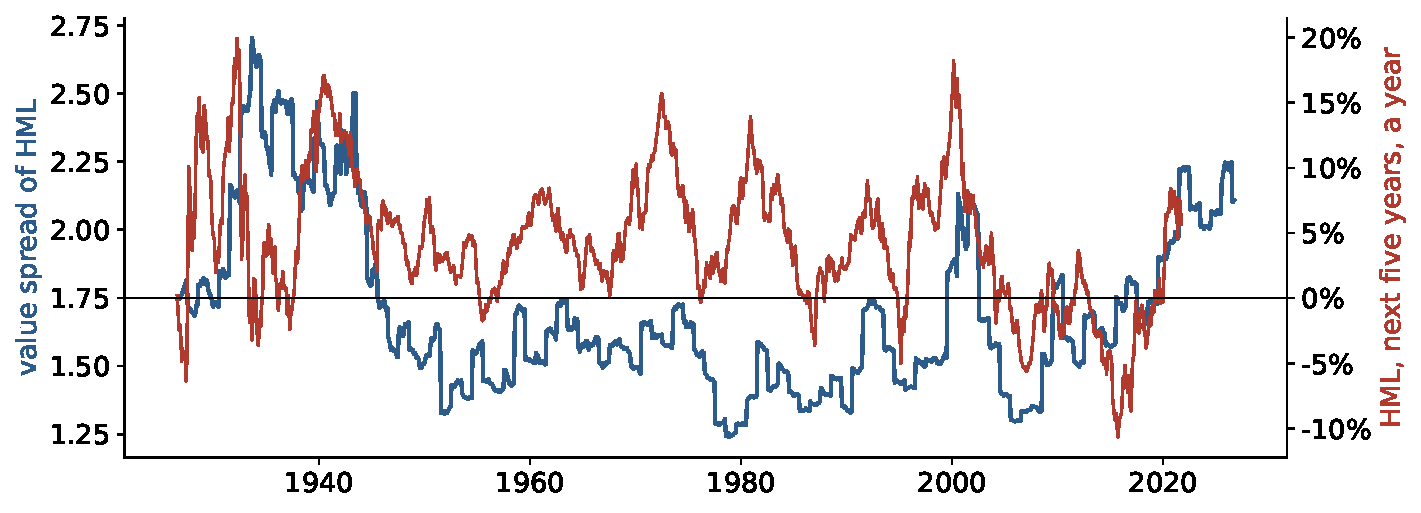
\includegraphics{figures/cs_value_spread.pdf}}
\end{center}
\begin{itemize}
\item High: what the factor buys is unusually cheap against what it sells. The Gordon logic again: a high return ahead, or low relative growth.
\vskip 4pt
\item HML, 1926--2026: correlation with the next five years' return \textcolor{red}{0.26}. D/P's was 0.35.
\vskip 4pt
\item Cohen, Polk and Vuolteenaho (2003); Haddad, Kozak and Santosh (2020)
\end{itemize}
\end{frame}

\begin{frame}[label=vstable]{Value spreads beat the historical average, out of sample}
\vskip 2pt
\begin{center}
\renewcommand{\arraystretch}{1.25}
\begin{tabular}{lcccccc}
\toprule
 & & in sample & \multicolumn{3}{c}{out of sample, from 1980} \\
\cmidrule(lr){3-3} \cmidrule(lr){4-6}
factor & from & $t$, HAC & $R^{2}$ & Sharpe, buy and hold & Sharpe, timed \\
\midrule
HML & 1926 & 1.2 & 0.6\% & 0.25 & 0.28 \\
SMB & 1926 & 1.3 & 0.4\% & 0.03 & 0.04 \\
RMW & 1963 & 2.4 & 0.7\% & 0.46 & 0.44 \\
CMA & 1963 & 3.8 & \textcolor{red}{1.1\%} & 0.38 & \textcolor{red}{0.49} \\
\bottomrule
\end{tabular}
\end{center}
{\small Next month's factor return on this month's value spread. Out of sample exactly as for D/P: each month, fit on the past only. Timed: forecast over $\gamma\sigma^{2}$.}
\vskip 6pt
\begin{itemize}
\item All four beat the historical average out of sample. D/P did not: you will measure it from 1980 for homework.
\vskip 4pt
\item Small $R^{2}$s and small gains, except CMA. But four tries, each with a reason, not a search.
\vskip 4pt
\item Careful: the book-to-market here uses last December's price. At today's price the $R^{2}$ is about zero. \hfill \hyperlink{appendix_vs}{\beamerbutton{Which price?}}
\end{itemize}
\end{frame}

\begin{frame}{What could break it}
\vskip 8pt
\begin{itemize}
\item \textbf{Book value misses what growth firms own.} Spending on R\&D, software and brands is expensed, so their book equity is too low and they look expensive for reasons that say nothing about future returns.
\vskip 10pt
\item \textbf{If that grows over time, the spread drifts up and stays up.} The same failure as buybacks for D/P: the signal's average moves.
\vskip 10pt
\item \textbf{The spread is near its widest since the 1940s.} Cheap value, or mismeasured book? The regression cannot tell you.
\end{itemize}
\vskip 14pt
\begin{beamercolorbox}[rounded=true,sep=7pt,center]{box1}
A price ratio is a good signal only if what is in the denominator means the same thing over time
\end{beamercolorbox}
\end{frame}

%================================================================== SEARCHING
\begin{frame}{Beyond prices: 24 tries}
\vskip 4pt
Six factors, 1980--2026. Four simple signals for each, its own:
\vskip 8pt
\begin{center}
\renewcommand{\arraystretch}{1.3}
\begin{tabular}{ll}
\toprule
signal & the idea \\
\midrule
return last month & factor momentum, short run \\
return over the last 12 months & factor momentum \\
return three to five years ago & reversal: what did well long ago does badly \\
volatility last month & last class: does risk forecast the return? \\
\bottomrule
\end{tabular}
\end{center}
\vskip 10pt
\begin{itemize}
\item Forecasting regression for each: next month's return on this month's signal
\vskip 4pt
\item Run it on 1980--2002, then again on 2003--2026. A real signal should work in both.
\end{itemize}
\end{frame}

\begin{frame}{Searching finds things. Some of them are real.}
\begin{columns}[c]
\begin{column}{0.56\textwidth}
\adjustbox{max width=\textwidth, max height=0.76\textheight}{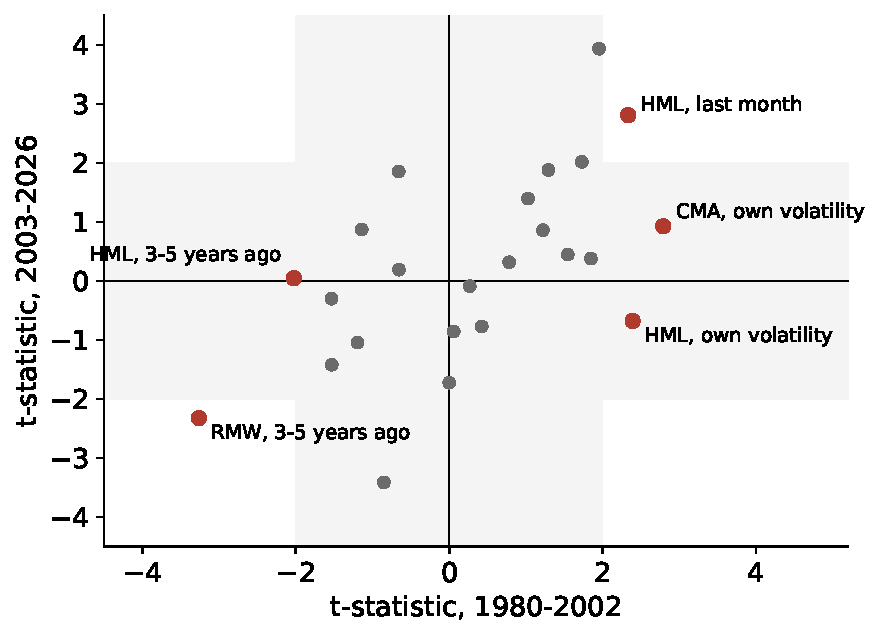
\includegraphics{figures/cs_tstats.pdf}}
\end{column}
\begin{column}{0.42\textwidth}
\begin{itemize}
\item In the first half, 5 of the 24 have $|t| > 2$. Luck alone gives about one.
\vskip 8pt
\item Of the best five (red), \textcolor{red}{two} still work in the second half
\vskip 8pt
\item The other three were the first half's luck
\vskip 8pt
\item With 24 tries you would have bet on all five
\end{itemize}
\end{column}
\end{columns}
\end{frame}

\begin{frame}{What holds up: factor momentum}
\vskip 2pt
\begin{center}
\renewcommand{\arraystretch}{1.25}
\begin{tabular}{lccc}
\toprule
signal: last month's return & $t$, 1980--2002 & $t$, 2003--2026 & \\
\midrule
HML & 2.3 & 2.8 & \textcolor{red}{both} \\
RMW & 2.0 & 3.9 & \textcolor{red}{both} \\
CMA & 1.7 & 2.0 & \\
UMD & $-0.7$ & 1.9 & \\
Market & 0.8 & 0.3 & \\
SMB & 0.1 & $-0.9$ & \\
\bottomrule
\end{tabular}
\end{center}
\vskip 8pt
\begin{itemize}
\item Factors that did well last month tend to do well this month. Gupta and Kelly (2019); Ehsani and Linnainmaa (2022)
\vskip 4pt
\item Hold a factor only after a positive year: a higher Sharpe ratio for five of the six, 1981--2026. Not for UMD.
\vskip 4pt
\item One signal, several factors, both halves: that is what a real one looks like
\end{itemize}
\end{frame}

%================================================================== WHAT TO TAKE AWAY
\begin{frame}{Why timing risk is easier than timing returns}
\vskip 4pt
\begin{center}
\renewcommand{\arraystretch}{1.4}
\adjustbox{max width=\textwidth}{\begin{tabular}{lcc}
\toprule
 & timing risk & timing returns \\
\midrule
what you forecast & next month's volatility & next month's return \\
how well, $R^{2}$ & \textcolor{red}{50\%} & \textcolor{red}{0.3\%}, in sample \\
what you need to be true & the return does not rise with risk & the signal's average stays put \\
how often it broke here & by factor & by decade \\
\bottomrule
\end{tabular}}
\end{center}
\vskip 10pt
\begin{itemize}
\item The race from \emph{Capital Allocation III} again: a signal against the noise in estimating it
\vskip 6pt
\item Volatility forecasts win that race easily. Return forecasts barely enter it.
\end{itemize}
\end{frame}

\begin{frame}{How to test a timing idea}
\vskip 6pt
\begin{enumerate}
\item \textbf{The signal is known at $t$.} Last year's dividends, last December's book value, last month's volatility. Check the index, as in \emph{Capital Allocation III}.
\vskip 6pt
\item \textbf{Out of sample, month by month.} Fit on the past only. Compare with the historical average, not with zero.
\vskip 6pt
\item \textbf{Count the overlap.} Long-horizon returns: HAC $t$-statistics, or count the independent periods.
\vskip 6pt
\item \textbf{Count your tries, and prefer a reason.} 24 tries give about one $|t| > 2$ for free.
\vskip 6pt
\item \textbf{Then ask for alpha.} Against buy and hold with the same beta, after costs. And check which years earned it.
\end{enumerate}
\end{frame}

%================================================================== THE NOTEBOOK
\begin{frame}{Notebook, exercise 1: the dividend yield, at three horizons}
\[ r_{t \to t+h} \;=\; a \;+\; b\cdot \frac{D}{P}\Big|_{t} \;+\; u_{t+h} \]
\vskip 2pt
\begin{itemize}
\item The market, 1926--2024. Plot D/P against the return over the next five years
\vskip 6pt
\item Run the regression for the next month, the next year and the next five years
\vskip 6pt
\item Two $t$-statistics for each: as usually computed, and HAC with \texttt{maxlags} equal to the horizon
\end{itemize}
\vskip 12pt
\begin{beamercolorbox}[rounded=true,sep=7pt,center]{box1}
Look for: which $t$ would you report? How many five-year periods do not overlap?
\end{beamercolorbox}
\end{frame}

\begin{frame}{Notebook, exercise 2: out of sample}
\[ R^{2}_{\text{OOS}} \;=\; 1 - \frac{\sum \left(r - \text{forecast}\right)^{2}}{\sum \left(r - \text{average}\right)^{2}} \]
\vskip 2pt
\begin{itemize}
\item The loop: each month from 1950, fit on the past, forecast next month, keep the historical average
\vskip 6pt
\item Then the out-of-sample $R^{2}$, for the whole period and for three sub-periods. Positive means D/P beat the average.
\vskip 6pt
\item Setup has the same two steps as functions. The later exercises use them.
\end{itemize}
\vskip 12pt
\begin{beamercolorbox}[rounded=true,sep=7pt,center]{box1}
Look for: in which periods D/P beat the historical average, and when it stopped
\end{beamercolorbox}
\end{frame}

\begin{frame}{Notebook, exercise 3: trade it}
\[ x_{t} \;=\; \frac{\text{forecast}_{t}}{\gamma\,\sigma^{2}} \qquad \sigma^{2}\text{: the market's variance before 1950, held fixed} \]
\vskip 2pt
\begin{itemize}
\item The weight on the market each month, from exercise 2's forecasts. Negative means short.
\vskip 6pt
\item Against buy and hold \emph{with the same average weight}: Sharpe ratio and volatility, by period, and the cumulative return of both
\vskip 6pt
\item Then the alpha: regress the timing return on the market's, from 1950 and again from 1956
\end{itemize}
\vskip 12pt
\begin{beamercolorbox}[rounded=true,sep=7pt,center]{box1}
Look for: does $\gamma$ change the Sharpe ratio? When did timing lose ground, and what was D/P doing then?
\end{beamercolorbox}
\end{frame}

\begin{frame}{Notebook, exercise 4: each factor's value spread}
\[ \text{VS}_{t} \;=\; \log \frac{B}{M}\Big|_{\text{long},\,t} \;-\; \log \frac{B}{M}\Big|_{\text{short},\,t} \]
\vskip 2pt
\begin{itemize}
\item Yours: the value spread of HML, from its two book-to-market columns
\vskip 6pt
\item Then exercises 1 to 3 again, in a loop over HML, SMB, RMW and CMA: the in-sample $t$, the out-of-sample $R^{2}$ from 1980, and timing against buy and hold
\end{itemize}
\vskip 12pt
\begin{beamercolorbox}[rounded=true,sep=7pt,center]{box1}
Look for: which factors beat the historical average, and by how much. Compare with D/P.
\end{beamercolorbox}
\end{frame}

\begin{frame}{Notebook, exercise 5: 24 tries}
\vskip 4pt
\begin{itemize}
\item Four signals for each of the six factors: last month, last 12 months, three to five years ago, own volatility
\vskip 6pt
\item The forecasting regression on 1980--2002, then on 2003--2026
\vskip 6pt
\item Count the $|t| > 2$ in the first half. Follow the best five into the second.
\end{itemize}
\vskip 14pt
\begin{beamercolorbox}[rounded=true,sep=7pt,center]{box1}
Look for: how many survive, and which signal works for several factors in both halves
\end{beamercolorbox}
\end{frame}

\begin{frame}{Takeaways}
\begin{enumerate}
\item Timing returns needs a forecast of the mean, the input data teaches you least about.
\vskip 4pt
\item The dividend yield looks strong at long horizons because the observations overlap. Allow for it and the evidence is thin.
\vskip 4pt
\item A real monthly $R^{2}$ of 1\% would be worth a lot. Out of sample, D/P's is negative.
\vskip 4pt
\item Factors' value spreads do better out of sample, but the gains are small and depend on how book-to-market is measured.
\vskip 4pt
\item Search finds things. Factor momentum survives the check on data it was not found in.
\end{enumerate}
\vskip 10pt
\begin{beamercolorbox}[rounded=true,sep=7pt]{box1}
\textbf{Homework: start later.} Rerun the out-of-sample test for D/P with forecasts from 1980, and set it against the value spreads. One number, three sentences.
\end{beamercolorbox}
\end{frame}

%================================================================== APPENDIX
\appendix
\begin{frame}
\begin{center}
{\Large Appendix}
\end{center}
\end{frame}

\begin{frame}[label=appendix_hac]{A1: Why overlapping returns inflate $t$}
\begin{center}
\adjustbox{max width=\textwidth}{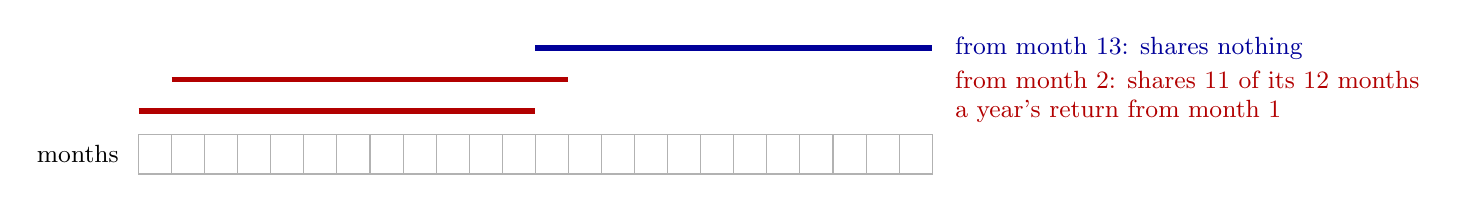
\begin{tikzpicture}[x=0.42cm, y=0.5cm]
\foreach \i in {0,...,23} \draw[gray!60] (\i,0) rectangle (\i+1,1);
\node[anchor=east, font=\small] at (-0.3,0.5) {months};
\draw[red!70!black, line width=2pt] (0,1.6) -- (12,1.6); \node[anchor=west, font=\small, red!70!black] at (24.4,1.6) {a year's return from month 1};
\draw[red!70!black, line width=2pt] (1,2.4) -- (13,2.4); \node[anchor=west, font=\small, red!70!black] at (24.4,2.4) {from month 2: shares 11 of its 12 months};
\draw[blue!60!black, line width=2pt] (12,3.2) -- (24,3.2); \node[anchor=west, font=\small, blue!60!black] at (24.4,3.2) {from month 13: shares nothing};
\end{tikzpicture}}
\end{center}
\vskip 6pt
\begin{itemize}
\item Neighbouring long-horizon returns are mostly the same months, so their errors move together
\vskip 4pt
\item The usual formula treats them as new information each month, and overstates $t$
\vskip 4pt
\item HAC (Newey--West) standard errors allow the errors to be correlated over the overlap. Here, \texttt{cov\_type='HAC'} with \texttt{maxlags} equal to the horizon.
\end{itemize}
\hfill \hyperlink{reg}{\beamerreturnbutton{Back}}
\end{frame}

\begin{frame}[label=appendix_ct]{A2: Where the small-$R^{2}$ formula comes from}
Let next month's excess return be $r = \mu_{t} + \varepsilon$, with the forecast $\mu_{t}$ varying around $\bar\mu$, and $\sigma$ the return's volatility.
\vskip 6pt
\begin{itemize}
\item $R^{2}$ is the share of the return's variance that the forecast explains: $\operatorname{Var}(\mu_{t}) = R^{2}\sigma^{2}$
\vskip 4pt
\item The timer holds $x_{t} \propto \mu_{t}$. Its squared Sharpe ratio is the buy-and-hold one, $\bar\mu^{2}/\sigma^{2}$, plus what the forecast adds, $R^{2}$, over the risk left, $1 - R^{2}$
\vskip 4pt
\item A monthly $R^{2}$ of 1\% and a monthly Sharpe ratio of $0.40/\sqrt{12} = 0.12$: $\;(0.0133 + 0.01)/0.99 = 0.024$, a year $\sqrt{12 \times 0.024} = 0.53$
\end{itemize}
\vskip 6pt
{\small An approximation: it assumes the forecast is right on average, and ignores the error in estimating it, which is the whole problem out of sample.}
\hfill \hyperlink{ct}{\beamerreturnbutton{Back}}
\end{frame}

\begin{frame}[label=appendix_vs]{A3: The value spread: which price?}
\begin{itemize}
\item Ken French's book-to-market divides book equity by market value \emph{last December}. The portfolios form each June, so in June 2026 the price in the ratio is from December 2025.
\vskip 4pt
\item Rebuilt at today's price: book over June's price, then rolled forward each month with the leg's own return
\end{itemize}
\vskip 2pt
\begin{center}
\renewcommand{\arraystretch}{1.2}
\begin{tabular}{lcccc}
\toprule
 & \multicolumn{2}{c}{last December's price} & \multicolumn{2}{c}{today's price} \\
\cmidrule(lr){2-3} \cmidrule(lr){4-5}
factor & $t$, HAC & $R^{2}$ from 1980 & $t$, HAC & $R^{2}$ from 1980 \\
\midrule
HML & 1.2 & 0.6\% & 0.8 & 0.0\% \\
SMB & 1.3 & 0.4\% & $-0.3$ & $-0.4\%$ \\
RMW & 2.4 & 0.7\% & 1.6 & 0.3\% \\
CMA & 3.8 & 1.1\% & 1.3 & \textcolor{red}{$-0.5\%$} \\
\bottomrule
\end{tabular}
\end{center}
\vskip 2pt
\begin{itemize}
\item The gap between the two moves with the factor's return over the past year (correlation about 0.75). A stale price builds in factor momentum, and that is much of what forecasts.
\end{itemize}
\hfill \hyperlink{vstable}{\beamerreturnbutton{Back}}
\end{frame}

\begin{frame}{A4: Data, and what to be careful about}
\begin{itemize}
\item \textbf{Market, 1926--2024.} CRSP value-weighted index with and without dividends, which gives the dividend yield. T-bills from Ken French.
\vskip 5pt
\item \textbf{Value spreads.} Ken French's 2$\times$3 sorts, the ones behind the factors: HML and SMB from 1926, RMW and CMA from 1963. Each leg's book-to-market is the average over its portfolios. None for momentum: French does not publish it.
\vskip 5pt
\item \textbf{The out-of-sample tests.} Each month uses only pairs of (signal, next month's return) that were complete by then. The benchmark is the historical average up to that month.
\vskip 5pt
\item \textbf{The strategies} hold $\sigma$ fixed at its value before the test starts, so all of the timing comes from the forecast. No costs; the market strategy is short a third of the time.
\vskip 5pt
\item \textbf{The 24 signals} are not the only 24 one could try, and the halves were chosen by date, not by looking.
\end{itemize}
\end{frame}

\end{document}
